
\documentclass{article}
\usepackage[utf8]{inputenc}
\usepackage{pgfplots}
\pgfplotsset{compat=1.18}
\usepackage{parskip}  % This will help for paragraph spacing, if needed
\begin{document}

\section*{\textbf{CS330 SPRING 2024 COURSE ASSESSMENT}}
Instructor \\
\\
\textbf{Part I - Performance Indicators, student outcomes and levels of focus.} \\
\\
CS6 : Apply computer science theory and software development fundamentals to produce computing-based solutions. \\
\\
\begin{tabular}{|p{0.333\textwidth}|p{0.333\textwidth}|p{0.333\textwidth}|}\hline
Course Activities & Program Indicator & Description \\ \hline
final exam grade & Understand the optimization processes, if necessary, to implement a better solution. & f \\ \hline
TSP assignment & Understand the optimization processes, if necessary, to implement a better solution. & gd \\ \hline
electric Dijkstra assignment & Choose the best algorithm / data structure, to solve a given computing problem. & f \\ \hline
\end{tabular} \\
\\
\\
\textbf{Part II - Rubrics.} \\
\\
\begin{tabular}{|p{0.200\textwidth}|p{0.200\textwidth}|p{0.200\textwidth}|p{0.200\textwidth}|p{0.200\textwidth}|}\hline
Course Activity & Exemplary & Satisfactory & Developing & Unsatisfactory \\ \hline
final exam grade & a & d & s & d \\ \hline
TSP assignment & s & d & s & d \\ \hline
electric Dijkstra assignment & a & d & d & s \\ \hline
\end{tabular} \\
\\
\\
\textbf{Part III – Outcome Assessment.} \\
\\
\begin{tabular}{|p{0.200\textwidth}|p{0.200\textwidth}|p{0.200\textwidth}|p{0.200\textwidth}|p{0.200\textwidth}|}\hline
ID & Exemplary & Satisfactory & Developing & Unsatisfactory \\ \hline
final exam grade & 3 & 5 & 4 & 6 \\ \hline
TSP assignment & 3 & 3 & 4 & 5 \\ \hline
electric Dijkstra assignment & 2 & 3 & 4 & 5 \\ \hline
Cumulative Attaiment & 8 & 11 & 12 & 16 \\ \hline
Level of Attainment for CS6 & 17.02\% & 23.40\% & 25.53\% & 34.04\% \\ \hline
\end{tabular} \\
\\
\\

    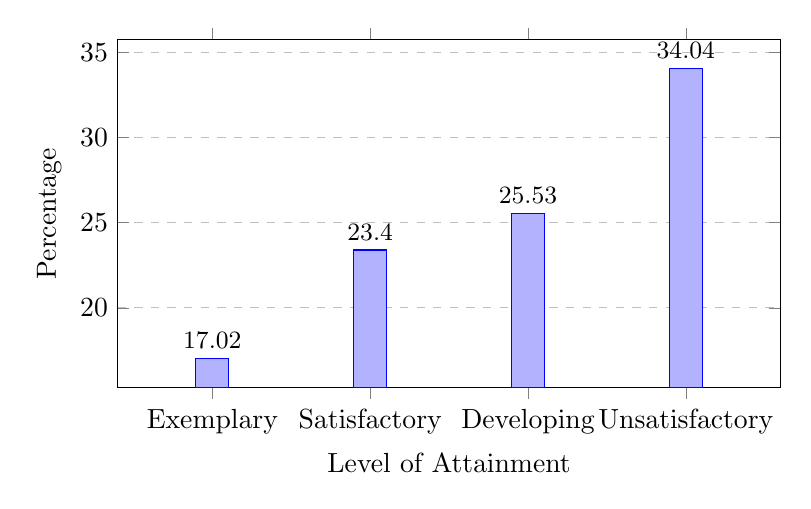
\begin{tikzpicture}
    \begin{axis}[
        ybar,
        width=10cm,
        height=6cm,
        enlarge x limits=0.2, 
        xlabel={Level of Attainment},
        ylabel={Percentage},
        symbolic x coords={Exemplary, Satisfactory, Developing, Unsatisfactory},
        xtick={Exemplary, Satisfactory, Developing, Unsatisfactory}, 
        xtick distance=0.1, 
        ymajorgrids=true,
        grid style=dashed,
        nodes near coords, % Display numbers near bars
        every node near coord/.append style={font=\small, text=black}, 
        bar width=12pt, 
    ]
    \addplot coordinates {(Exemplary, 17.02) (Satisfactory, 23.4) (Developing, 25.53) (Unsatisfactory, 34.04)};
    \end{axis}
    \end{tikzpicture}
     \\
\\
\\
\textbf{Part IV – Analysis.} \\
\\
\parbox{\textwidth}{\raggedright aaa}
\end{document}
